% ------------------------------------------------------------------
% Bragg band gaps in a LEGO sonic crystal along GammaX and GammaM
% LFE, Module I -- final report (English)
% Compile with: pdflatex report.tex   (twice, for the cross-references)
% Figures 2, 3, A1-A3 are read from the files named in \figfile{...};
% if a file is missing, a grey placeholder box is drawn instead.
% ------------------------------------------------------------------
\documentclass[9pt,a4paper,twocolumn]{extarticle}
\usepackage[a4paper,top=1.3cm,bottom=1.4cm,left=1.3cm,right=1.3cm,columnsep=0.55cm]{geometry}
\usepackage[utf8]{inputenc}
\usepackage[english]{babel}
\usepackage{amsmath,amssymb}
\usepackage{siunitx}
\usepackage{graphicx,xcolor,booktabs,caption,titlesec}
\usepackage{tikz}
\usetikzlibrary{arrows.meta,decorations.pathreplacing}
\usepackage[colorlinks=true,allcolors=blue!50!black]{hyperref}
\usepackage{float}
\usetikzlibrary{arrows.meta}
\newcommand{\pbreak}{\par\vspace{3pt}}

\sisetup{range-phrase={--},range-units=single,separate-uncertainty=true,per-mode=symbol}
\newcommand{\umm}{\milli\metre}
\newcommand{\ucm}{\centi\metre}
\newcommand{\uHz}{\hertz}
\newcommand{\ukHz}{\kilo\hertz}
\newcommand{\udB}{\decibel}
\newcommand{\ums}{\metre\per\second}
\newcommand{\us}{\second}

\newcommand{\GX}{\ensuremath{\Gamma X}}
\newcommand{\GM}{\ensuremath{\Gamma M}}
\newcommand{\fB}{\ensuremath{f_B}}
\newcommand{\finf}{\ensuremath{f_{\mathrm{inf}}}}
\newcommand{\fsup}{\ensuremath{f_{\mathrm{sup}}}}
\newcommand{\rip}{\mathrm{rip}}

\captionsetup{font=footnotesize,skip=3pt,labelfont=bf,labelsep=period,justification=justified}
\titleformat{\section}{\large\bfseries}{\thesection}{0.6em}{}
\titlespacing*{\section}{0pt}{6pt plus 2pt}{3pt}
\titleformat{\paragraph}[runin]{\normalfont\normalsize\bfseries\itshape}{}{0em}{}[.\ ]
\titlespacing*{\paragraph}{0pt}{3pt plus 1pt}{0.5em}
\setlength{\parindent}{1.2em}
\setlength{\parskip}{0pt}
\setlength{\textfloatsep}{6pt plus 2pt minus 2pt}\setlength{\floatsep}{5pt plus 2pt minus 2pt}\setlength{\intextsep}{5pt}

% external figure, or a grey placeholder if the file does not exist yet
\newcommand{\figfile}[3]{%
  \IfFileExists{#1}{\includegraphics[width=#2]{#1}}%
  {\fcolorbox{gray}{gray!10}{\parbox[c][#3][c]{\dimexpr#2-2\fboxsep-2\fboxrule\relax}{\centering\footnotesize [placeholder: \detokenize{#1}]}}}}

\begin{document}

\twocolumn[{%
\begin{center}
  {\Large\bfseries Bragg band gaps in a LEGO sonic crystal along $\Gamma X$ and $\Gamma M$}\\[4pt]
  {\small Afonso Duarte (ist1118524) \;·\; Filipe Marcelino (ist1117896) \;·\; Inês Ferreira (ist1117578) \;·\; José Santos (ist1)\\
   LFE, Module I \;·\; Group Ornitorrinco \;·\; Instituto Superior Técnico, October 2026}
\end{center}
\vspace{2pt}
\noindent\colorbox{gray!12}{\parbox{\dimexpr\textwidth-2\fboxsep\relax}{\small
\textbf{Abstract.}\ A sonic crystal blocks sound in a band of frequencies, the band gap, expected near $f_B=c/(2d)$, with $d$ the spacing between planes of scatterers. We measured the transmission of white noise (spectrum with crystal divided by spectrum without crystal) through square lattices of $2\times2$ LEGO columns, with lattice constant $a=32$--$56$\,mm and $N=1$--$11$ rows, along \GX{} and \GM{} (lattice rotated by $45^\circ$), and compared it with a plane-wave expansion (PWE). Along \GX{} the lower gap edge agrees with the PWE within $1.3\sigma$ for $a\le48$\,mm but not for $a=56$\,mm ($3.9\sigma$); the gap does not scale as $1/a$ ($\chi^2/\nu=15$), and the attenuation grows linearly with $N$, by $1.45\pm0.29$ to $1.98\pm0.41$\,dB per row ($a=40$--$56$\,mm). Rotating the crystal to \GM{} raises the lower edge by a factor $1.27$--$1.45$, consistent with $\sqrt2$ within $2\sigma$. The precision is limited by the reference measurement and by sound bypassing the crystal, and we find no evidence of a complete gap.
}}
\vspace{4pt}
}]

\section{Introduction}
A sonic crystal is a periodic array of rigid obstacles in air. Reflections from successive planes of obstacles, separated by $d$, add in phase when $\lambda=2d$, and around
\begin{equation}
f_B=\frac{c}{2d},\qquad d=a\ (\GX),\qquad d=a/\sqrt2\ (\GM)
\end{equation}
a band gap opens \cite{mart,kush}: at the edge of the Brillouin zone, $k=\pi/d$, the standing waves with maximum pressure on the planes of bricks and in the air between them no longer have the same frequency, and between the two, $\finf<f_B<\fsup$, no wave propagates. Inside the gap $k=\pi/d+i\kappa$ and the pressure decays as $e^{-\kappa x}$; after $N$ rows the attenuation in decibels is
\begin{equation}
D(N)=\alpha N,\qquad \alpha=20\log_{10}(e)\,\kappa d.
\end{equation}
The position and width of the gap depend on the filling fraction $ff=s^2/a^2$ (0.24 to 0.08 here): the bricks slow the sound down, $c_{\rm eff}\simeq c/\sqrt{1+ff}$ \cite{krokhin}, and the gap moves below $f_B$, more so for smaller $a$. The bands are computed by solving $\nabla\!\cdot(\rho^{-1}\nabla p)+\omega^2p/(\rho c^2)=0$ with $p$ written as a Bloch wave (PWE, 225 plane waves, Appendix~B). We tested, along \GX{} and \GM, the gap edges, their dependence on $a$, the linear attenuation in $N$, and whether the gaps of the two directions overlap (complete gap).

\section{Method}

\paragraph{Experimental set-up}
The crystal is a square lattice of columns (Fig.~\ref{fig:setup}), each one a stack of $2\times2$ LEGO bricks (side $s = \SI{15.8}{\milli\metre}$) on a LEGO baseplate. The lattice constant $a$ is the centre-to-centre distance between neighbouring columns; since the studs of the baseplate are \SI{8}{\milli\metre} apart, $a$ is a multiple of \SI{8}{\milli\metre}.

Along $\Gamma X$ the rows are at $d = a$. Only this spacing along the propagation direction sets the Bragg frequency, $f_B = c/(2d)$, and it was the only one changed: the lateral spacing and the enclosure were kept fixed, so the entrance is always $W = 18$ studs (\SI{144}{\milli\metre}) wide. Along $\Gamma M$ the lattice is rotated by \SI{45}{\degree} (rows alternating between 4 and 3 bricks, with 3 at the entrance) and the two spacings can no longer be chosen separately: the planes are at $d = a/\sqrt{2}$ and the columns within a plane at $L = \sqrt{2}\,a = 2d$, so $f_B = c/L$. Increasing $a$ therefore widens the lattice laterally as well, and so the entrance, which holds three columns, grows with it: $W = 14$, 17 and 20 studs, i.e.\ 112, 136 and \SI{160}{\milli\metre}, for $a = 32$, 40 and \SI{48}{\milli\metre}.

The crystal is enclosed by LEGO walls and roof and placed in a cardboard box with foam around it. A Bluetooth loudspeaker $\approx\SI{70}{\centi\metre}$ from the crystal face emits white noise, with frequencies between 500 and \SI{12000}{\hertz}, for \SI{10}{\second}, and a USB microphone \SI{5}{\centi\metre} behind the crystal records the sound. The loudspeaker distance satisfies the plane-wave criterion (Appendix~B).

\begin{figure}[H]
  \centering
  \resizebox{\columnwidth}{!}{%
  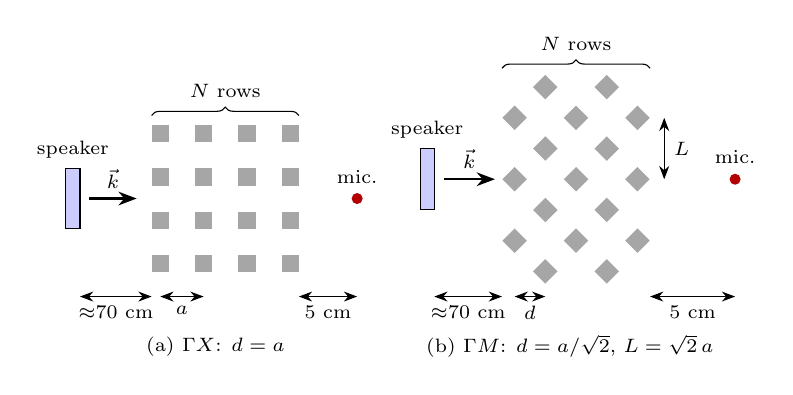
\begin{tikzpicture}[>=Stealth, font=\scriptsize]
    % ================= (a) Gamma X =================
    \begin{scope}
      \foreach \i in {0,1,2,3}{\foreach \j in {0,1,2,3}{
        \fill[gray!70] ({1.2+0.55*\i-0.11},{0.1+0.55*\j-0.11}) rectangle ++(0.22,0.22);}}
      \draw[fill=blue!20] (0,0.54) rectangle (0.18,1.31);
      \node[above] at (0.09,1.31) {speaker};
      \draw[->,thick] (0.3,0.925) -- (0.9,0.925) node[midway,above] {$\vec k$};
      \fill[red!70!black] (3.7,0.925) circle (0.07);
      \node[above] at (3.7,0.99) {mic.};
      \draw[decorate,decoration={brace,amplitude=3pt}] (1.09,1.98) -- (2.96,1.98)
        node[midway,above=3pt] {$N$ rows};
      \draw[<->] (0.18,-0.32) -- node[below] {$\approx$70 cm} (1.09,-0.32);
      \draw[<->] (1.2,-0.32) -- node[below] {$a$} (1.75,-0.32);
      \draw[<->] (2.96,-0.32) -- node[below] {5 cm} (3.7,-0.32);
      \node at (1.9,-0.95) {(a) $\Gamma X$: $d=a$};
    \end{scope}
    % ====== (b) Gamma M: rotated lattice, brick vertex facing the speaker ======
    \begin{scope}[shift={(4.5,0)}]
      \foreach \k in {0,2,4}{\foreach \j in {0,1,2}{
        \begin{scope}[shift={({1.2+0.39*\k},{0.39+0.78*\j})},rotate=45]
          \fill[gray!70] (-0.11,-0.11) rectangle (0.11,0.11);
        \end{scope}}}
      \foreach \k in {1,3}{\foreach \j in {0,1,2,3}{
        \begin{scope}[shift={({1.2+0.39*\k},{0.78*\j})},rotate=45]
          \fill[gray!70] (-0.11,-0.11) rectangle (0.11,0.11);
        \end{scope}}}
      \draw[fill=blue!20] (0,0.78) rectangle (0.18,1.56);
      \node[above] at (0.09,1.56) {speaker};
      \draw[->,thick] (0.3,1.17) -- (0.95,1.17) node[midway,above] {$\vec k$};
      \fill[red!70!black] (4.0,1.17) circle (0.07);
      \node[above] at (4.0,1.24) {mic.};
      \draw[decorate,decoration={brace,amplitude=3pt}] (1.04,2.58) -- (2.92,2.58)
        node[midway,above=3pt] {$N$ rows};
      \draw[<->] (3.1,1.17) -- node[right] {$L$} (3.1,1.95);
      \draw[<->] (0.18,-0.32) -- node[below] {$\approx$70 cm} (1.04,-0.32);
      \draw[<->] (1.2,-0.32) -- node[below] {$d$} (1.59,-0.32);
      \draw[<->] (2.92,-0.32) -- node[below] {5 cm} (4.0,-0.32);
      \node at (1.9,-0.95) {(b) $\Gamma M$: $d=a/\sqrt2$, $L=\sqrt2\,a$};
    \end{scope}
  \end{tikzpicture}}
  \caption{Set-up seen from above (not to scale). Each column is a stack of $2\times2$ LEGO bricks on a LEGO baseplate. (a)~$\Gamma X$: aligned columns. (b)~$\Gamma M$: lattice rotated by \SI{45}{\degree}, with a brick vertex facing the loudspeaker and rows alternating between 4 and 3 bricks. $a$: distance between columns $d$: distance between planes; $L$: period within a plane.}
  \label{fig:setup}
\end{figure}

\paragraph{Parameters varied and repetitions}
We varied $a = 32$, 40, 48 and \SI{56}{\milli\metre} along $\Gamma X$ and $a = 32$, 40 and \SI{48}{\milli\metre} along $\Gamma M$, and the number of rows $N$, removing one row at a time from the microphone side ($N = 10 \to 1$ along $\Gamma X$ and $N = 11 \to 1$ along $\Gamma M$, except along $\Gamma M$ with $a = \SI{32}{\milli\metre}$, where $N = 1$ was not measured). The loudspeaker, the microphone and the volume were kept fixed. Each configuration had 5 recordings, for a total of 72 configurations and 360 recordings, of which 16 were excluded for saturation or Bluetooth dropouts. The 4 sessions (1 and 6 October along $\Gamma X$, 12 and 13 October along $\Gamma M$) took place at $\theta = \SI{20.5}{\celsius}$ and \SI{20.0}{\celsius} ($\pm\,\SI{1}{\celsius}$), which gives $c = \SI{343.5 \pm 0.6}{\metre\per\second}$ and \SI{343.2 \pm 0.6}{\metre\per\second}.

\paragraph{Quantity measured and data processing}
We measured the relative transmission
\begin{equation}
  T(f) = 10\log_{10}\!\left[\frac{\bar P_{\mathrm{crystal}}(f)}{\bar P_{\mathrm{ref}}(f)}\right]\ (\si{\decibel}),
\end{equation}
where $P$ is the power spectral density of the recorded signal, analysed from \SI{500}{\hertz} to \SI{12}{\kilo\hertz}, and the reference is the same set-up without columns. The division removes the response of the loudspeaker, the microphone and the room.
\pbreak
\emph{Spectra.} $P$ was computed with Welch's method (Hann window, 4096 points, $\Delta f = \SI{11.7}{\hertz}$ (Frequency resolution of the spectrum) at a sampling rate of \SI{48}{\kilo\hertz}) on the segment \SIrange{0.8}{10.3}{\second} of each recording, which excludes the Bluetooth delay.
\pbreak
\emph{Smoothing.} To reduce the statistical fluctuations of the spectrum, which are amplified when dividing two spectra, each $P$ was smoothed in power, i.e.\ the value at each frequency $f$ was replaced by the mean power in a window around $f$ (and not by the mean in dB, to avoid biasing the result). The window is 1/6 of an octave wide (an octave is an interval in which the frequency doubles), i.e.\ it goes from $f/1.06$ to $f\cdot1.06$ ($\pm\SI{6}{\percent}$ of $f$).
\pbreak
\emph{Reference.} The reference was measured for each value of $a$ at the start (and also at the end, along $\Gamma M$) of the measurements. For each $a$ we used, among the references of the session, the one that makes $T(f)$ flattest in the control band (see below); the others enter the uncertainty associated with the reference.

\paragraph{Control band}
As a check of the measurement, $T$ should be constant and close to \SI{0}{\decibel} in the band $0.35$--$0.70\,f_0$, with $f_0 = c/(2a)$ along both directions. This band lies at frequencies below the first gap of the lattice, where the crystal is practically transparent. Along $\Gamma M$ we use $f_0 = c/(2a)$ and not $f_B = c/(2d)$, because the band $0.35$--$0.70\,f_B$ would reach the $\Gamma X$ gap.

\section{Analysis}
From each $T(f)$ we extract: the base level $T_0$ (median in the control band $0.35$--$0.70\,c/(2a)$, transparent along both directions) and the \emph{ripple} (robust deviation of $T$ in that band, where $T$ should be flat); the gap, a continuous region with $T<T_0-\SI{6}{\udB}$ that touches $0.75$--$1.25\,f_B$, whose threshold crossings are \finf{} and \fsup{} (the gap ``closes'' if $\fsup<1.5f_B$); and the depth $D=T_0-\langle T\rangle_{f_B\pm10\%}$. The windows are in units of $f_B$, so the calculations are the same along both directions.

\emph{Uncertainties.} For each number, $\sigma^2=\sigma_{\rm est}^2+\sigma_{\rm rip}^2+\sigma_{\rm ref}^2\,(+\sigma_{\rm res}^2)$: dispersion of the 5 repetitions ($/\sqrt5$, almost always negligible), propagated ripple ($0.92\times$ripple in $D$; ripple$/|dT/df|$ at the edges), dispersion among the references of the same day, and $\Delta f/\sqrt{12}=\SI{3.4}{\uHz}$. Per block, the frequencies are the weighted mean over $N\ge4$, with $\sigma^2=\sigma_{\rm disp}^2+\sigma_{\rm sys}^2$: the systematic part (ripple and reference, common to the whole block) does not decrease with averaging. Fits are weighted least squares ($\sigma_a=\SI{0.1}{\umm}$ through effective variance); if $\chi^2/\nu>1$ the uncertainties are multiplied by $\sqrt{\chi^2/\nu}$. The theory has an uncertainty from the brick side ($\pm\SI{0.1}{\umm}$) and from the PWE truncation ($0.5\,\%$). Comparisons use $z=|x-x_0|/\sqrt{\sigma_x^2+\sigma_0^2}$.

\section{Results}
\emph{Gap edges.} Along \GX{} there is a well-defined gap for $N\ge4$ for all $a$ (Fig.~\ref{fig:T}); it closes in 27 of the 28 measurements with $N\ge4$. The edges are in Table~\ref{tab:main}: for $a\le\SI{48}{\umm}$, \finf{} agrees with the PWE within $1.3\sigma$ and \fsup{} within $2.6\sigma$; for $a=\SI{56}{\umm}$ both lie above ($z=3.9$ and 3.6).

\begin{figure}[t]
\centering
\figfile{fig2_transmission.pdf}{\columnwidth}{7.2cm}
\caption{Relative transmission for $a=\SI{48}{\umm}$. Grey: PWE gap; red: measured edges (mean over $N\ge4$). Along \GX{} the gap closes; along \GM{} lateral diffraction starts at $f_B$ and $T$ does not return to 0. All $a$ in Appendix~A.}
\label{fig:T}
\end{figure}

\begin{figure}[t]
\centering
\figfile{fig3_depth.pdf}{\columnwidth}{3.6cm}
\caption{Depth $D$ at $f_B\pm10\,\%$ versus number of rows, with the line $D=\alpha N+b$ fitted for each $a$ (slopes in Table~\ref{tab:main}).}
\label{fig:D}
\end{figure}

\begin{table}[t]
\centering
\caption{Results per block (mean over $N\ge4$) versus the PWE. Frequencies in Hz; $\alpha$ in dB/row. $^\dagger$~The gap does not close. $^\ddagger$~Only 14--38\,\% of the $f_B\pm10\,\%$ window lies inside the theoretical gap: compares orders of magnitude only.}
\label{tab:main}
\scriptsize
\setlength{\tabcolsep}{2.6pt}
\begin{tabular}{@{}llrrrrrrrrrr@{}}
\toprule
 & $a$ & $f_B$ & \multicolumn{3}{c}{\finf} & \multicolumn{3}{c}{\fsup} & \multicolumn{2}{c}{$\alpha$}\\
 \cmidrule(lr){4-6}\cmidrule(lr){7-9}\cmidrule(l){10-11}
 & mm & & meas. & PWE & $z$ & meas. & PWE & $z$ & meas. & PWE\\
\midrule
\GX & 32 & 5367 & 3806(84) & 3892 & 1.0 & 5923(191) & 6037 & 0.6 & 0.81(39) & 5.4\\
    & 40 & 4294 & 3586(151) & 3387 & 1.3 & 5117(227) & 4752 & 1.6 & 1.98(41) & 4.0\\
    & 48 & 3578 & 2969(102) & 2988 & 0.2 & 4230(135) & 3880 & 2.6 & 1.45(29) & 2.8\\
    & 56 & 3067 & 2917(62)  & 2666 & 3.9 & 3722(124) & 3271 & 3.6 & 1.53(11) & 1.9\\
\midrule
\GM & 32 & 7584 & 5500(271) & 6180 & 2.5 & ---$^\dagger$ & 6990 & --- & 0.73(20) & 0.1$^\ddagger$\\
    & 40 & 6067 & 4557(173) & 5109 & 3.1 & 7149(410) & 5818 & 3.2 & 0.81(28) & 0.5$^\ddagger$\\
    & 48 & 5056 & 4040(93)  & 4385 & 3.6 & ---$^\dagger$ & 4942 & --- & 1.30(17) & 0.6$^\ddagger$\\
\bottomrule
\end{tabular}
\end{table}

\emph{Dependence on $a$.} The line $f_c=m/(2a)$ through the origin gives $m=\SI{339\pm15}{\ums}$, compatible with $c=\SI{343.5\pm0.6}{\ums}$ ($z=0.3$), but with $\chi^2/\nu=15.4$ ($p=5\times10^{-10}$): on average the centre is at $f_B$, but it is not proportional to $1/a$. The free line describes the points ($\chi^2/\nu=1.4$) with $m=\SI{229\pm20}{\ums}$ and intercept $\SI{1283\pm231}{\uHz}$. For \finf{} the same holds: through the origin $m=\SI{278\pm20}{\ums}$ with $\chi^2/\nu=30$ (Appendix~A). The PWE gives $f_c/f_B=0.925$--$0.968$.

\emph{Attenuation.} Along \GX{} the depth grows linearly with $N$ (Fig.~\ref{fig:D}): for $a=40$, 48 and \SI{56}{\umm} the intercept is $b=-0.2\pm2.0$, $-0.6\pm1.9$ and $-0.3\pm0.6$\,dB (compatible with 0, as Eq.~(2) predicts) and $\chi^2/\nu=0.3$--$1.4$. For $a=\SI{32}{\umm}$, $D$ saturates at $\approx\SI{13}{\udB}$ from $N=4$ and the line gives $b=5.1\pm2.9$\,dB. The measured $\alpha$ is 15, 50, 53 and 80\,\% of the PWE value for $a=32$--\SI{56}{\umm}.

\emph{Direction \GM.} \finf{} is 8--11\,\% below the PWE ($z=2.5$--$3.6$) and the gap closes in only 3/8, 5/8 and 4/8 of the measurements ($a=32$, 40, \SI{48}{\umm}). The ratio $\finf(\GM)/\finf(\GX)$ is $1.445(78)$, $1.271(72)$ and $1.360(56)$, versus $\sqrt2$ (Bragg; $z=0.4$, 2.0, 1.0) and 1.59, 1.51, 1.47 (PWE; $z=1.8$, 3.3, 1.9). The measured overlap $\fsup(\GX)-\finf(\GM)$ is $423\pm331$, $560\pm286$ and $191\pm163$\,Hz, less than $2\sigma$ above zero; the PWE gives $-143$, $-357$ and $-505$\,Hz (no complete gap).

\section{Discussion}
\emph{\GX.} A PWE for an infinite 2D crystal of rigid rods describes the lower edge for $a\le\SI{48}{\umm}$ without free parameters, and the gap below $f_B$ for $a=\SI{32}{\umm}$ ($ff=0.24$) is consistent with the slowing of sound by the bricks. This is what makes the line through the origin fail: the slope $\SI{339\pm15}{\ums}$ would be ``the speed of sound'' if the gap were always at $f_B$, but the $\chi^2/\nu$ shows that it is not. The measured trend in $f_c/f_B$ is stronger than the PWE one, especially for $a=\SI{56}{\umm}$, where the theoretical gap is only \SI{600}{\uHz} wide, comparable to the $1/6$-octave smoothing ($\approx\SI{350}{\uHz}$ at \SI{3}{\ukHz}), and the crossings of a fixed threshold no longer coincide with the band edges. The $a=\SI{40}{\umm}$ block mixed two sessions, hence the larger systematic uncertainty.

\emph{Attenuation.} $D\propto N$ with $b\approx0$ is the signature of the evanescent Bloch wave \cite{sanchez}. But the crystal is only \SI{3.8}{\ucm} tall and \SIrange{11}{16}{\ucm} wide: some sound goes over the top and around the sides, which imposes a ceiling of $\approx$\SIrange{13}{15}{\udB}. The larger the theoretical $\alpha$, the sooner the ceiling is reached: hence the measured/theory fraction grows from 15\,\% ($a=32$) to 80\,\% ($a=56$).

\emph{\GM.} With the source at $\sim\SI{70}{\ucm}$ and a narrow crystal, sound that crosses the crystal obliquely, close to \GX, whose gap is lower, reaches the microphone: $T$ starts to drop before the \GM{} gap and \finf{} comes out low. Above $f_B$ the rows, of period $L=\sqrt2a$, diffract sound sideways from $c/L=f_B$ and the sound no longer reaches the on-axis microphone; the gap stays ``open''. For the same reasons the measured overlap does not prove a complete gap.

\emph{Limitations.} The reference dominates the error: moving the loudspeaker or the microphone by \SI{1}{\ucm} changes the spectrum by several dB, and the ripple of $T$ (0.5--\SI{8}{\udB}) is much larger than the dispersion of the repetitions. A rigid lid, a wider crystal and repeated reassemblies would reduce and measure these effects.

\section{Conclusion}
A LEGO crystal with $a=32$--\SI{56}{\umm} has a Bragg gap along \GX{} whose lower edge agrees with the PWE within $1.3\sigma$ for $a\le\SI{48}{\umm}$, and which does not scale as $1/a$ because of the filling fraction. The attenuation is linear in $N$, $\alpha\approx1.5$--\SI{2}{\udB}/row, limited to $\approx\SI{15}{\udB}$ by sound that goes around the crystal. Along \GM{} the gap appears about $\sqrt2$ higher, but the lower edge is 8--11\,\% below the PWE and the gap does not close, because of oblique propagation and lateral diffraction; there is no evidence of a complete gap.

\begin{thebibliography}{9}\footnotesize
\setlength{\itemsep}{1pt}
\bibitem{mart} R. Martínez-Sala \emph{et al.}, Nature \textbf{378}, 241 (1995).
\bibitem{kush} M. S. Kushwaha \emph{et al.}, Phys. Rev. Lett. \textbf{71}, 2022 (1993).
\bibitem{sanchez} J. V. Sánchez-Pérez \emph{et al.}, Phys. Rev. Lett. \textbf{80}, 5325 (1998).
\bibitem{krokhin} A. A. Krokhin, J. Arriaga, L. N. Gumen, Phys. Rev. Lett. \textbf{91}, 264302 (2003).
\bibitem{welch} P. D. Welch, IEEE Trans. Audio Electroacoust. \textbf{15}, 70 (1967).
\bibitem{bev} P. R. Bevington, D. K. Robinson, \emph{Data Reduction and Error Analysis for the Physical Sciences}, McGraw-Hill (2003).
\end{thebibliography}

\pbreak
% =================== APPENDIX (does not count towards the 2 pages) ===================
\onecolumn
\appendix
\section*{A\quad Additional data and measurements}
\begin{figure}[h]
\centering
\figfile{figA1_all_blocks.pdf}{\textwidth}{7.5cm}
\caption{$T-T_0$ for all blocks with $N\ge4$ (top: \GX; bottom: \GM). Band: PWE gap; red dashed: onset of lateral diffraction, $c/L$; dotted: threshold $T_0-\SI{6}{\udB}$. Along \GM{} there are no measurements with $a=\SI{56}{\umm}$ and $N\ge4$.}
\end{figure}
\begin{figure}[h]
\centering
\figfile{figA2_fit_1_2d.pdf}{0.95\textwidth}{8cm}
\caption{\finf{} and $f_c$ (mean over $N\ge4$ for each $a$) versus $x=1/(2d)$, with the line through the origin and the free line; below, normalised residuals. Dashed: $f=c\,x$.}
\end{figure}
\begin{figure}[h]
\centering
\figfile{figA3_directions.pdf}{0.95\textwidth}{9cm}
\caption{Top: \GX{} ($N=10$) and \GM{} ($N=11$) for the same $a$, with the measured gaps (bands) and $f_B$ (dashed). Bottom: $\finf/f_B$ and $f_c/f_B$ along both directions.}
\end{figure}

\begin{table}[h]
\centering
\caption{All measurements. ``rip.'': ripple of $T$ in the control band (dB); ``$k$/5 rep.'': repetitions used; ``ref.\ other $a$'': reference from the same session but from another block. Total uncertainty $\sigma^2=\sigma_{\rm est}^2+\sigma_{\rm rip}^2+\sigma_{\rm ref}^2\,(+\sigma_{\rm res}^2)$. The components are also in \texttt{tabela.csv}.}
\scriptsize
\setlength{\tabcolsep}{4pt}
\renewcommand{\arraystretch}{0.93}
\begin{tabular}{llrlcrrrrl}
\toprule
dir & $a$ (mm) & $N$ & day & reference & rip. & $D$ (dB) & \finf{} (Hz) & \fsup{} (Hz) & notes\\
\midrule
$\Gamma X$ & 32 & 1 & 10-01 & ref\_a32 & 4.2 & $-1.3\pm4.3$ & --- & --- &  \\
$\Gamma X$ & 32 & 2 & 10-01 & ref\_a32 & 6.2 & $0.1\pm6.0$ & --- & --- &  \\
$\Gamma X$ & 32 & 3 & 10-01 & ref\_a32 & 7.6 & $3.5\pm7.2$ & $5529\pm889$ & $5609\pm599$ &  \\
$\Gamma X$ & 32 & 4 & 10-01 & ref\_a32 & 1.7 & $11.4\pm2.1$ & $3947\pm195$ & $5768\pm1747$ & 4/5 rep. \\
$\Gamma X$ & 32 & 5 & 10-01 & ref\_a32 & 1.8 & $8.0\pm2.7$ & $3846\pm133$ & $5622\pm161$ &  \\
$\Gamma X$ & 32 & 6 & 10-01 & ref\_a32 & 2.2 & $12.7\pm2.8$ & $3795\pm67$ & $5802\pm109$ &  \\
$\Gamma X$ & 32 & 7 & 10-01 & ref\_a32 & 1.7 & $13.5\pm2.3$ & $3781\pm70$ & $6431\pm165$ &  \\
$\Gamma X$ & 32 & 8 & 10-01 & ref\_a32 & 2.1 & $13.4\pm2.8$ & $3880\pm91$ & $6028\pm181$ &  \\
$\Gamma X$ & 32 & 9 & 10-01 & ref\_a32 & 1.5 & $9.9\pm1.8$ & $3794\pm79$ & $5981\pm893$ &  \\
$\Gamma X$ & 32 & 10 & 10-01 & ref\_a32 & 1.6 & $13.1\pm2.0$ & $3773\pm78$ & $5890\pm919$ & 4/5 rep. \\
\midrule
$\Gamma X$ & 40 & 1 & 10-06 & ref\_a56 & 3.1 & $-4.2\pm3.1$ & --- & --- & 4/5 rep., ref. other $a$ \\
$\Gamma X$ & 40 & 2 & 10-06 & ref\_a56 & 5.4 & $3.9\pm5.1$ & $4538\pm944$ & $4713\pm254$ & ref. other $a$ \\
$\Gamma X$ & 40 & 3 & 10-06 & ref\_a56 & 1.0 & $6.0\pm1.2$ & $3196\pm330$ & $4832\pm126$ & 4/5 rep., ref. other $a$ \\
$\Gamma X$ & 40 & 4 & 10-06 & ref\_a56 & 1.2 & $8.9\pm1.6$ & $3474\pm168$ & $5677\pm114$ & ref. other $a$ \\
$\Gamma X$ & 40 & 5 & 10-06 & ref\_a56 & 4.2 & $7.2\pm4.1$ & $3625\pm327$ & $4783\pm163$ & ref. other $a$ \\
$\Gamma X$ & 40 & 6 & 10-06 & ref\_a56 & 2.0 & $14.5\pm2.0$ & $3525\pm122$ & $4818\pm271$ & ref. other $a$ \\
$\Gamma X$ & 40 & 7 & 10-01 & ref\_a40 & 4.4 & $19.0\pm5.3$ & $3696\pm157$ & $4875\pm185$ &  \\
$\Gamma X$ & 40 & 8 & 10-01 & ref\_a40 & 4.7 & $10.1\pm4.8$ & $3833\pm213$ & $5510\pm462$ &  \\
$\Gamma X$ & 40 & 9 & 10-01 & ref\_a40 & 1.9 & $13.2\pm3.2$ & $3669\pm330$ & $4854\pm111$ &  \\
$\Gamma X$ & 40 & 10 & 10-01 & ref\_a40 & 2.2 & $18.2\pm4.1$ & $3556\pm101$ & --- & does not close \\
\midrule
$\Gamma X$ & 48 & 1 & 10-06 & ref\_a48 & 1.9 & $-1.1\pm2.7$ & --- & --- &  \\
$\Gamma X$ & 48 & 2 & 10-06 & ref\_a48 & 2.4 & $2.5\pm2.7$ & --- & --- & 4/5 rep. \\
$\Gamma X$ & 48 & 3 & 10-06 & ref\_a48 & 2.3 & $4.6\pm2.7$ & $3600\pm502$ & $3770\pm1598$ &  \\
$\Gamma X$ & 48 & 4 & 10-06 & ref\_a48 & 2.3 & $5.2\pm2.9$ & $3613\pm568$ & $4173\pm364$ &  \\
$\Gamma X$ & 48 & 5 & 10-06 & ref\_a48 & 2.7 & $8.7\pm2.8$ & $2883\pm125$ & $4157\pm260$ &  \\
$\Gamma X$ & 48 & 6 & 10-06 & ref\_a48 & 2.5 & $9.6\pm2.9$ & $2970\pm100$ & $4071\pm161$ & 4/5 rep. \\
$\Gamma X$ & 48 & 7 & 10-06 & ref\_a48 & 2.0 & $9.4\pm2.6$ & $2982\pm98$ & $4093\pm130$ & 4/5 rep. \\
$\Gamma X$ & 48 & 8 & 10-06 & ref\_a48 & 2.0 & $10.7\pm2.1$ & $2974\pm83$ & $4306\pm112$ &  \\
$\Gamma X$ & 48 & 9 & 10-06 & ref\_a48 & 2.3 & $9.6\pm2.8$ & $3019\pm79$ & $4332\pm96$ &  \\
$\Gamma X$ & 48 & 10 & 10-06 & ref\_a48 & 2.8 & $15.0\pm2.7$ & $2850\pm135$ & $4210\pm123$ &  \\
\midrule
$\Gamma X$ & 56 & 1 & 10-06 & ref\_a56 & 0.8 & $0.7\pm0.7$ & --- & --- &  \\
$\Gamma X$ & 56 & 2 & 10-06 & ref\_a56 & 1.1 & $2.7\pm1.0$ & --- & --- & 4/5 rep. \\
$\Gamma X$ & 56 & 3 & 10-06 & ref\_a56 & 0.5 & $4.4\pm0.5$ & $3018\pm50$ & $3142\pm230$ &  \\
$\Gamma X$ & 56 & 4 & 10-06 & ref\_a56 & 1.1 & $5.7\pm1.0$ & $2993\pm75$ & $3418\pm200$ &  \\
$\Gamma X$ & 56 & 5 & 10-06 & ref\_a56 & 1.6 & $9.1\pm1.5$ & $2912\pm72$ & $3607\pm133$ & 4/5 rep. \\
$\Gamma X$ & 56 & 6 & 10-06 & ref\_a56 & 1.6 & $10.6\pm1.5$ & $2941\pm56$ & $3587\pm98$ & 4/5 rep. \\
$\Gamma X$ & 56 & 7 & 10-06 & ref\_a56 & 0.8 & $11.3\pm0.7$ & $2884\pm46$ & $3593\pm77$ &  \\
$\Gamma X$ & 56 & 8 & 10-06 & ref\_a56 & 1.3 & $11.0\pm1.2$ & $2979\pm47$ & $3993\pm103$ &  \\
$\Gamma X$ & 56 & 9 & 10-06 & ref\_a56 & 1.5 & $15.1\pm1.5$ & $2595\pm266$ & $3809\pm215$ &  \\
$\Gamma X$ & 56 & 10 & 10-06 & ref\_a56 & 1.0 & $13.3\pm0.9$ & $2821\pm58$ & $3886\pm85$ &  \\
\midrule
$\Gamma M$ & 32 & 2 & 10-13 & ref\_a32 & 1.6 & $3.3\pm1.5$ & $6288\pm297$ & $6883\pm150$ &  \\
$\Gamma M$ & 32 & 3 & 10-13 & ref\_a32 & 1.7 & $4.0\pm1.6$ & $5950\pm96$ & $6953\pm128$ &  \\
$\Gamma M$ & 32 & 4 & 10-13 & ref\_a32 & 2.0 & $3.9\pm1.8$ & $7871\pm1018$ & $8223\pm817$ & 4/5 rep. \\
$\Gamma M$ & 32 & 5 & 10-13 & ref\_a32 & 2.0 & $2.7\pm1.9$ & $6005\pm2114$ & $6989\pm120$ &  \\
$\Gamma M$ & 32 & 6 & 10-13 & ref\_a32 & 2.0 & $7.4\pm1.9$ & $6076\pm179$ & --- & does not close \\
$\Gamma M$ & 32 & 7 & 10-13 & ref\_a32 & 1.8 & $8.4\pm1.6$ & $5910\pm73$ & --- & 4/5 rep., does not close \\
$\Gamma M$ & 32 & 8 & 10-13 & ref\_a32 & 1.6 & $10.0\pm1.5$ & $4603\pm189$ & --- & does not close \\
$\Gamma M$ & 32 & 9 & 10-13 & ref\_a32 & 1.9 & $5.7\pm1.8$ & $4680\pm206$ & $8281\pm309$ &  \\
$\Gamma M$ & 32 & 10 & 10-13 & ref\_a32 & 1.9 & $8.7\pm1.8$ & $4581\pm141$ & --- & does not close \\
$\Gamma M$ & 32 & 11 & 10-13 & ref\_a32 & 2.4 & $9.2\pm2.2$ & $4664\pm353$ & --- & does not close \\
\midrule
$\Gamma M$ & 40 & 1 & 10-13 & ref\_a40\_fim & 5.3 & $-2.1\pm4.9$ & --- & --- &  \\
$\Gamma M$ & 40 & 2 & 10-13 & ref\_a40\_fim & 1.4 & $4.8\pm1.3$ & $6260\pm302$ & $6794\pm1291$ &  \\
$\Gamma M$ & 40 & 3 & 10-13 & ref\_a40\_fim & 1.9 & $6.1\pm1.7$ & $4712\pm335$ & $5756\pm593$ & 4/5 rep. \\
$\Gamma M$ & 40 & 4 & 10-13 & ref\_a40\_fim & 1.4 & $7.7\pm1.3$ & $4633\pm101$ & --- & 4/5 rep., does not close \\
$\Gamma M$ & 40 & 5 & 10-13 & ref\_a40\_fim & 1.9 & $10.2\pm1.7$ & $4695\pm445$ & $7151\pm209$ &  \\
$\Gamma M$ & 40 & 6 & 10-13 & ref\_a40\_fim & 1.9 & $12.4\pm1.7$ & $4706\pm213$ & $8699\pm493$ &  \\
$\Gamma M$ & 40 & 7 & 10-13 & ref\_a40\_fim & 2.3 & $11.4\pm2.2$ & $4535\pm210$ & $6865\pm1507$ &  \\
$\Gamma M$ & 40 & 8 & 10-13 & ref\_a40\_fim & 2.0 & $14.1\pm1.8$ & $4544\pm175$ & $8655\pm429$ &  \\
$\Gamma M$ & 40 & 9 & 10-13 & ref\_a40\_fim & 2.5 & $11.1\pm2.3$ & $4624\pm342$ & --- & does not close \\
$\Gamma M$ & 40 & 10 & 10-13 & ref\_a40\_fim & 2.6 & $7.4\pm2.4$ & $4616\pm184$ & --- & does not close \\
$\Gamma M$ & 40 & 11 & 10-13 & ref\_a40\_fim & 2.6 & $9.9\pm2.4$ & $4206\pm165$ & $6696\pm177$ & 4/5 rep. \\
\midrule
$\Gamma M$ & 48 & 1 & 10-12 & ref\_a48\_fim & 1.4 & $0.4\pm1.5$ & --- & --- &  \\
$\Gamma M$ & 48 & 2 & 10-12 & ref\_a48\_fim & 1.3 & $4.2\pm1.8$ & $5838\pm656$ & --- & 4/5 rep. \\
$\Gamma M$ & 48 & 3 & 10-12 & ref\_a48\_fim & 1.2 & $6.5\pm1.7$ & $3896\pm112$ & --- &  \\
$\Gamma M$ & 48 & 4 & 10-12 & ref\_a48\_fim & 1.3 & $8.3\pm1.6$ & $4148\pm215$ & $6287\pm557$ &  \\
$\Gamma M$ & 48 & 5 & 10-12 & ref\_a48\_fim & 1.9 & $8.5\pm2.3$ & $4131\pm176$ & $6232\pm769$ &  \\
$\Gamma M$ & 48 & 6 & 10-12 & ref\_a48\_fim & 1.0 & $9.6\pm1.2$ & $3966\pm61$ & --- & does not close \\
$\Gamma M$ & 48 & 7 & 10-12 & ref\_a48\_fim & 1.7 & $7.0\pm2.2$ & $4314\pm76$ & $5068\pm144$ &  \\
$\Gamma M$ & 48 & 8 & 10-12 & ref\_a48\_fim & 2.7 & $8.7\pm2.7$ & $4360\pm236$ & $6941\pm973$ &  \\
$\Gamma M$ & 48 & 9 & 10-12 & ref\_a48\_fim & 0.9 & $13.6\pm1.3$ & $3945\pm50$ & --- & does not close \\
$\Gamma M$ & 48 & 10 & 10-12 & ref\_a48\_fim & 1.2 & $14.8\pm1.4$ & $3990\pm85$ & --- & does not close \\
$\Gamma M$ & 48 & 11 & 10-12 & ref\_a48\_fim & 2.1 & $12.2\pm3.0$ & $4260\pm188$ & --- & does not close \\
\bottomrule
\end{tabular}
\end{table}

\clearpage
\section*{B\quad Calibrations and derivations}
\paragraph{Speed of sound.} $c(\theta)=331.3\sqrt{1+\theta/273.15}$\,m/s, $\sigma_c=c\,\sigma_\theta/[2(273.15+\theta)]=\SI{0.6}{\ums}$ for $\sigma_\theta=\SI{1}{\celsius}$.

\paragraph{Plane-wave Criterion.} The loudspeaker emits approximately spherical waves. For the wave at the crystal entrance to be treated as plane, the distance $r$ from the loudspeaker to the entrance must be large compared with the entrance width $W$. The loudspeaker faces the centre of the entrance, so its edges are at $W/2$ from the axis and are reached after an extra path, relative to the centre, of $\delta = \sqrt{r^2 + (W/2)^2} - r \approx W^2/(8r)$. This extra path corresponds to a phase difference of $360^\circ\,\delta/\lambda$ across the entrance, and we require $\delta \le \lambda/10$ (at most $36^\circ$), which gives
\begin{equation}
  r \ge \frac{1.25\,W^2}{\lambda_{\min}},
\end{equation}
where $\lambda_{\min} = c/f_{\max}$ is the smallest wavelength used in the analysis: $\delta$ does not depend on frequency, but $\lambda$ decreases with it, so the condition is most demanding at the highest frequency. The highest frequency we use is the upper gap edge, which in Table~1 is at most $1.21\,f_B$ ($a = \SI{56}{\milli\metre}$), so we take $f_{\max} = 1.2 f_B$, i.e.\ $\lambda_{\min} = 2d/1.2$. Along $\Gamma X$, $W = 18$ studs $= \SI{144}{\milli\metre}$ for all $a$; along $\Gamma M$, $W = 14$, 17 and 20 studs (112, 136 and \SI{160}{\milli\metre}) for $a = 32$, 40 and \SI{48}{\milli\metre}.

\begin{table}[htbp]
  \centering
  \caption{Minimum distance $r_{\min} = 1.25\,W^2/\lambda_{\min}$, with $\lambda_{\min} = 2d/1.2$ (upper edge of the gap), and margin with respect to $r = \SI{70}{\centi\metre}$.}
  \label{tab:B1}
  \begin{tabular}{l S[table-format=2.0] S[table-format=2.1] S[table-format=3.0] S[table-format=2.1] S[table-format=2.1] S[table-format=1.2]}
    \toprule
    {Lattice} & {$a$ (mm)} & {$d$ (mm)} & {$W$ (mm)} & {$\lambda_{\min}$ (mm)} & {$r_{\min}$ (cm)} & {$\SI{70}{\centi\metre}/r_{\min}$} \\
    \midrule
    $\Gamma X$ & 32 & 32.0 & 144 & 53.3 & 48.6 & 1.44 \\
    $\Gamma X$ & 40 & 40.0 & 144 & 66.7 & 38.9 & 1.80 \\
    $\Gamma X$ & 48 & 48.0 & 144 & 80.0 & 32.4 & 2.16 \\
    $\Gamma X$ & 56 & 56.0 & 144 & 93.3 & 27.8 & 2.52 \\
    $\Gamma M$ & 32 & 22.6 & 112 & 37.7 & 41.6 & 1.68 \\
    $\Gamma M$ & 40 & 28.3 & 136 & 47.1 & 49.0 & 1.43 \\
    $\Gamma M$ & 48 & 33.9 & 160 & 56.6 & 56.6 & 1.24 \\
    \bottomrule
  \end{tabular}
\end{table}

In all configurations $r = \SI{70}{\centi\metre}$ exceeds $r_{\min}$, with a minimum margin of 1.24 ($\Gamma M$, $a = \SI{48}{\milli\metre}$).

\paragraph{Plane-wave expansion (PWE).} With $\sigma = 1/\rho$, $\eta = 1/(\rho c^2)$ and $p(\mathbf r) = e^{i\mathbf k\cdot\mathbf r}\sum_{\mathbf G} p_{\mathbf G}\, e^{i\mathbf G\cdot\mathbf r}$, $\mathbf G = \tfrac{2\pi}{a}(m,n)$, the wave equation gives, for each $\mathbf k$, the eigenvalue problem
\begin{equation*}
  \sum_{\mathbf G'}\sigma(\mathbf G-\mathbf G')\,(\mathbf k+\mathbf G)\cdot(\mathbf k+\mathbf G')\,p_{\mathbf G'}
  = \omega^2\sum_{\mathbf G'}\eta(\mathbf G-\mathbf G')\,p_{\mathbf G'},
\end{equation*}
with, for a square rod of side $s$, $\sigma(\mathbf G) = (\sigma_\text{t}-\sigma_\text{air})\,f\!f\,\operatorname{sinc}(G_xs/2)\operatorname{sinc}(G_ys/2)$ ($\mathbf G \neq 0$). We use $15^2 = 225$ waves (729 waves change the edges by 0.1--0.4\,\%). Only modes symmetric with respect to the plane containing the sound direction count (the antisymmetric ones are not excited by a wave arriving head-on). The gap is $f_\text{inf} = \max_k f_1(k)$, $f_\text{sup} = \min_k f_{n\ge2}(k)$, with $k$ from $\Gamma$ to X ($|\mathbf k| = \pi/a$) or from $\Gamma$ to M ($|\mathbf k| = \sqrt{2}\pi/a$). The attenuation comes from the inverse problem (given $\omega$, a complex $k$ comes out), $(k^2 M_2 + k M_1 + M_0)\,\mathbf p = 0$, linearised into a problem of double dimension; $\kappa$ is the smallest $|\operatorname{Im} k|$. With only the two waves $e^{\pm i\pi x/d}$, $f_\text{sup} - f_\text{inf} \propto |\sigma(2\pi/d)|$: the gap widens with the amount of brick per plane.

\paragraph{Effective medium.} At low frequency, $\kappa_{\rm eff}=(1-ff)\kappa$ and $\rho_{\rm eff}\simeq\rho(1+ff)/(1-ff)$ (rigid rods), hence $c_{\rm eff}=c/\sqrt{1+ff}$ and $f_{\rm gap}\approx f_B/\sqrt{1+ff}=0.90$, 0.93, 0.95, $0.96\,f_B$ for $a=32$--\SI{56}{\umm}.

\paragraph{Complete gap.} There is a gap along all directions if $\fsup(\GX)>\finf(\GM)$. Along \GM{} the diagonal of the brick (\SI{22.3}{\umm}) occupies almost the whole distance between planes ($a/\sqrt2=\SI{22.6}{\umm}$ for $a=\SI{32}{\umm}$): the medium looks almost uniform and the \GM{} gap is narrow, so the predicted ratio $\finf(\GM)/\finf(\GX)$ is 1.59, 1.51, 1.47 (and not $\sqrt2$) and there is no overlap for $2\times2$ bricks ($-\SI{7}{\uHz}$ even for $a=\SI{24}{\umm}$).

\paragraph{Uncertainty of the depth.} $D=T_0-M$; with $n_{\rm base}=\log_2(0.70/0.35)/(1/6)=6$ and $n_{\rm win}=\log_2(1.1/0.9)/(1/6)=1.74$ independent points, and the variance of the median being $\pi/2$ times that of the mean, $\mathrm{Var}\,D=\left(\frac\pi2\frac16+\frac1{1.74}\right)\sigma^2$, i.e.\ $\sigma_{\rm rip}(D)=0.92\times\mathrm{ripple}$. The dispersion of the references uses weights $w_k=1/\mathrm{rip}_k^2$: $\sigma_{\rm ref}^2=\sum_kw_k(x_k-x_0)^2/\sum_kw_k$.

\paragraph{Fits.} For $y=mx+b$ with $w_i=1/\sigma_i^2$: $m=(S\,S_{xy}-S_xS_y)/\Delta$, $b=(S_{xx}S_y-S_xS_{xy})/\Delta$, $\sigma_m^2=S/\Delta$, $\sigma_b^2=S_{xx}/\Delta$, $\Delta=S\,S_{xx}-S_x^2$ \cite{bev}; the uncertainty in $x$ enters through $\sigma_{i,\rm eff}^2=\sigma_{y,i}^2+(m\sigma_{x,i})^2$, minimising $\chi^2(m,b)$ numerically. If $\chi^2/\nu>1$, $\sigma\to\sqrt{\chi^2/\nu}\,\sigma$; uncertainties are never shrunk. The regressions were checked against \texttt{numpy.polyfit}, \texttt{scipy.optimize.curve\_fit} and \texttt{scipy.odr}.

\section*{C\quad Code}
Repository: \url{https://github.com/FM767/LFE-acoustics}.
\begin{itemize}\setlength{\itemsep}{0pt}
\item \texttt{cristal\_simples/} and \texttt{cristal\_lego\_g/cristal\_lego\_g/}: measurement apps (\GX{} and \GM; Python, \texttt{sounddevice}) with the measurement plan, quality control and the recordings (\texttt{projeto/dados/<step>/*.wav} + \texttt{meta.json}; repeated measurements in \texttt{\_antigos/}, which do not count).
\item \texttt{cristal\_lego\_g/analise 2.0/}: joint analysis of the two directions. \texttt{analise.py} (spectra, $T(f)$, quantities, uncertainties, fits), \texttt{teoria.py} (PWE), \texttt{graficos.py}, \texttt{app.py} (interface); results in \texttt{resultados/} (\texttt{resultados.txt}, \texttt{tabela.csv}, \texttt{ajustes.csv}, \texttt{teoria.txt}). All equations, in order, in \texttt{EQUACOES.md}.
\item \texttt{relatorio/}: this report. \texttt{fazer\_figuras.py} generates Figs.~2--3 and Table~A1 from \texttt{dados\_figuras/}; \texttt{dados\_figuras/curvas\_T.py} recomputes the curves of Fig.~2 from the \texttt{.wav} files (same method, numpy only).
\end{itemize}
Parameters: FS $=48000$, NPERSEG $=4096$, band 0.5--\SI{12}{\ukHz}, segment \SIrange{0.8}{10.3}{\us}, $1/6$-octave smoothing, \SI{6}{\udB} threshold, $\sigma_a=\SI{0.1}{\umm}$, $\sigma_\theta=\SI{1}{\celsius}$.

\section*{D\quad Use of AI}
We used Claude (Anthropic) as an assistant: in planning the experiment and choosing the parameters, in writing the measurement and analysis code (which we reviewed and tested: the regressions were compared with independent libraries and the coverage of the uncertainties by simulation) and in drafting this report from the results files. The set-up, the measurements, the decisions on what to measure and the verification of the numbers against \texttt{resultados.txt} and \texttt{teoria.txt} were done by us.

\end{document}
